\documentclass[11pt]{article}
\usepackage[margin=1in]{geometry}
\usepackage{enumitem}
\usepackage{graphicx}
\usepackage[hidelinks]{hyperref}
\usepackage[T1]{fontenc}
\usepackage[utf8]{inputenc}
\title{Agentic Video Generator\\Project Overview and Status}
\author{Video Agent Team}
\date{June 14, 2026}

\begin{document}
\maketitle

\section*{Executive Summary}
This project implements an agentic application that converts a user story into a generated video via a staged orchestration pipeline. The system currently supports persistent job tracking, asynchronous execution through a queue, ffmpeg-based assembly, and pluggable external providers for media and speech.

\section*{Current Architecture}
\begin{itemize}[leftmargin=*]
  \item \textbf{API Layer}: FastAPI endpoints for job creation and job status polling.
  \item \textbf{UI Layer}: Streamlit frontend for submission, polling, resume action, and video preview.
  \item \textbf{Orchestration Layer}: LangGraph state machine with nodes: director, storyboard, asset generation, voice synthesis, editor, and critic.
  \item \textbf{Persistence Layer}: Postgres for durable job state and metadata.
  \item \textbf{Queue Layer}: Redis list queue for asynchronous job processing.
  \item \textbf{Checkpoint Layer}: Redis (hot cache) + Postgres (durable) checkpoints for resumable runs.
  \item \textbf{Render Layer}: ffmpeg pipeline for scene composition and optional narration muxing.
  \item \textbf{Provider Layer}: Replicate adapters for image/video generation and ElevenLabs adapter for TTS, with local fallbacks.
\end{itemize}

\section*{Implemented Features (Status: Complete)}
\begin{enumerate}[leftmargin=*]
  \item FastAPI endpoints: \texttt{/generate}, \texttt{/jobs/\{job\_id\}}, \texttt{/jobs/\{job\_id\}/resume}.
  \item Typed schemas for \texttt{VideoPlan}, \texttt{ScenePlan}, and job status models.
  \item Queue-driven background execution using Redis.
  \item Postgres-backed persistent job store.
  \item Scene rendering with ffmpeg for image/video assets.
  \item Voiceover generation path with provider abstraction.
  \item Fallback behavior when provider credentials are absent.
  \item LangGraph checkpointing after each successful node execution.
  \item Streamlit UI with submit form, job polling, resume button, and video preview.
\end{enumerate}

\section*{Current Readiness and Unblocker}
\begin{itemize}[leftmargin=*]
  \item Core platform is operational for local fallback mode.
  \item Primary unblocker for production-like output quality is provider credential setup.
  \item Required keys to enable real generation providers:
  \begin{itemize}
    \item \texttt{REPLICATE\_API\_TOKEN} for image/video generation.
    \item \texttt{ELEVENLABS\_API\_KEY} for TTS narration.
  \end{itemize}
  \item \texttt{OPENAI\_API\_KEY} is optional in the current code path.
\end{itemize}

\section*{Environment and Infrastructure Status}
\begin{itemize}[leftmargin=*]
  \item Python virtual environment: configured at \texttt{.venv}.
  \item Application dependencies: installed via \texttt{requirements.txt}.
  \item ffmpeg: installed and available on host.
  \item Containers: Redis and Postgres started via \texttt{docker-compose.yml}.
\end{itemize}

\section*{Operational Notes}
If a health probe returns connection refused, the API process is not running. Restart the service with the project venv interpreter and retry \texttt{/health}.

\section*{Risks and Open Work}
\begin{itemize}[leftmargin=*]
  \item External model availability and model slug drift for provider APIs.
  \item Need stronger retry, idempotency, and dead-letter handling for production.
  \item Need dedicated worker process separation and deployment manifests.
  \item Need observability: tracing, metrics, and per-node latency/cost reporting.
\end{itemize}

\section*{Recommended Next Steps}
\begin{enumerate}[leftmargin=*]
  \item Add valid provider keys and run end-to-end quality test with real providers.
  \item Introduce separate API and worker services for production runtime.
  \item Add retry/backoff policy and failure classification per node.
  \item Add subtitle generation and timeline-level QA checks.
  \item Add CI checks and integration tests against Redis/Postgres.
\end{enumerate}

\appendix
\section*{Appendix A: Architecture Diagram}
\begin{center}
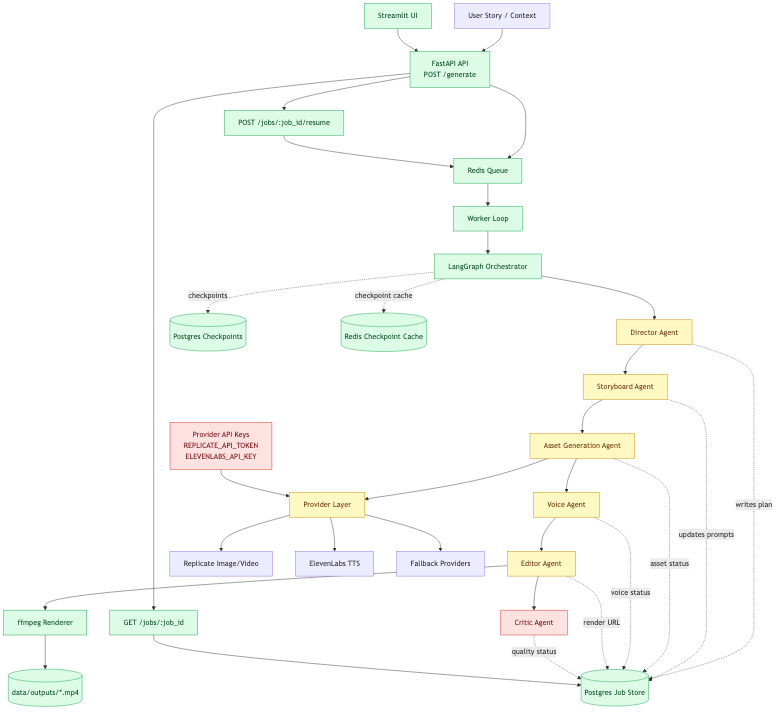
\includegraphics[width=\textwidth]{architecture.png}
\end{center}

\end{document}
